%************************************************
\chapter{Giant anisotropy of Gilbert damping in a Rashba honeycomb antiferromagnet} \label{ch:baglay}% $\mathbb{ZNR}$
\chaptermark{Giant anisotropy of Gilbert damping in a honeycomb antiferromagnet}

%************************************************
Giant Gilbert damping anisotropy is identified as a signature of strong Rashba spin-orbit coupling in a two-dimensional antiferromagnet on a honeycomb lattice. The phenomenon originates in spin-orbit induced splitting of conduction electron subbands that strongly suppresses certain spin-flip processes. As a result, the spin-orbit interaction is shown to support an undamped non-equilibrium dynamical mode that corresponds to an ultrafast in-plane N\'eel vector precession and a constant perpendicular-to-the-plane magnetization. The phenomenon is illustrated on the basis of a two dimensional $s$-$d$ like model. Spin-orbit torques and conductivity are also computed microscopically for this model. Unlike Gilbert damping these quantities are shown to reveal only a weak anisotropy that is limited to the semiconductor regime corresponding to the Fermi energy staying in a close vicinity of antiferromagnetic gap.

\vfill
Parts of this Chapter were published in Phys. Rev. \textbf{B} 101, 104403 (2020)\clearpage

\section{Introduction}
The N\'eel vector dynamics in an AFM is strongly affected by an interplay between different types of Gilbert dampings. Unlike in a simple single-domain ferromagnet with a single sublattice, the Gilbert damping in an AFM is generally different on different sublattices and includes spin pumping from one sublattice to another. A proper understanding of Gilbert damping is of key importance for addressing not only the mechanism of spin pumping but also domain wall motion, magnon lifetime, AFM resonance width and many other related phenomena \cite{PhysRevMaterials.1.061401, Kamra2018, Mahfouzi2018a, Yuan_2019, hals_phenomenology_2011}. It is also worth noting that spin pumping between two thin ferromagnetic layers with antiparallel magnetic orientations share many similarities with Gilbert damping in a bipartite AFM \cite{Heinrich2003,Tserkovnyak}. 

A conduction electron mechanism for Gilbert damping in collinear ferromagnet requires some spin-orbit interaction to be present. It is, therefore, commonly assumed that spin-orbit interaction of electrons naturally enhances the Gilbert damping. Contrary to this intuition, we show that Rashba spin-orbit coupling does generally suppress one of the Gilbert damping coefficients and leads to the appearance of undamped non-equilibrium N\'eel vector precession modes in the AFM. 

%%%%%%%%%%%%
%%% figure 1: lattice
%%%%%%%%%%%%
\begin{figure}
\centering
\centerline{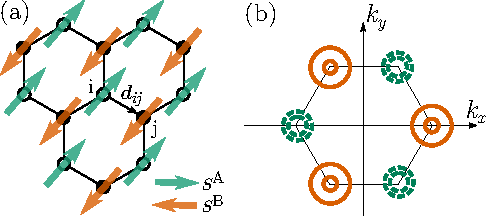
\includegraphics[width=\columnwidth]{{articles/misha_paper/fig1.pdf}}}
\caption{A model of Rashba honeycomb antiferromagnet with two sublattices, $A$ and $B$, and on-site exchange interaction between localized moments and conduction electrons (see Eq.~\ref{chap03:ex}). The large blue arrow represents the N\'eel vector vector, $\bm{n}$, that is in general, characterized by non-vanishing in-plane, $\bm{n}_\parallel$, and perpendicular-to-the-plane, $\bm{n}_\perp$, components. We refer to a specific coordinate system with $\hat{\bm{x}}$ axis chosen to be in the direction of $\bm{n}_\parallel$. 
}
\label{chap03:fig:lattice}
\end{figure}
%%%%%%%%%

The spin dynamics in a bipartite AFM is described in terms of two mutually orthogonal vector fields, $\bb{n}$ and $\bb{m}$. Even though the AFM ground state corresponds to $\bb{m}=0$, it is widely understood that no N\'eel dynamics is possible without formation of a small but finite nonequilibrium magnetization $\bb{m}$. It appears, however, that Gilbert damping terms associated with the time dynamics of $\bb{m}(t)$ and $\bb{n}(t)$ are essentially different from a microscopic point of view.

Indeed, the Gilbert damping that is proportional to $\partial_t\bb{n}$ is characterized by a coefficient $\alpha_n$, which is vanishing in the absence of spin-orbit interaction, much like it is the case in the ferromagnets. This behavior can be traced back to a spin-rotational symmetry of the collinear AFM. Indeed, the absolute value of $\bb{n}$ is conserved up to the order $m^2$. Thus, the dynamics of the N\'eel vector is essentially a rotation that does not change the conduction electron spectrum as far as the spin-rotation invariance is present. Breaking the spin-rotation symmetry by spin-orbit interaction induces, therefore, a finite $\alpha_n$, which is quadratic with respect to spin-orbit interaction strength.

In contrast, the Gilbert damping that is proportional to $\partial_t\bb{m}$ originates directly in the conduction electron scattering even in the absence of any spin-orbit interaction. The strength of the damping in a simple symmetric AFM is characterized by a coefficient $\alpha_m$, which is typically much larger than $\alpha_n$. As a rule, the spin-orbit interaction tends to suppress the coefficient $\alpha_m$ by restricting the ways in which electrons can damp their magnetic moments.  The condition $\alpha_m \gg \alpha_n$ has been indeed well documented in a metallic AFM \cite{PhysRevMaterials.1.061401, Mahfouzi2018a}. 

In this Chapter, we uncover the microscopic mechanism of strong and anisotropic Gilbert damping suppression due to the influence of spin-orbit interaction in a 2D AFM model on a honeycomb lattice. 

Below we focus mainly on the AFM in the regime of good metallic behavior, such that the Fermi energy of electrons exceeds by order of magnitude that of an effective $s$-$d$ exchange coupling between electron spins and localized AFM magnetic momenta.  In this case, the transition to the highly anisotropic regime takes place provided the characteristic spin-orbit energy $\lambda$ exceeds the scale $\hslash/\tau$, where $\tau$ is the electron scattering time. Alternatively, one may think of characteristic spin-orbit length becoming smaller than the mean free path of conduction electrons.  We show here that the splitting of 2D Fermi surfaces by spin-orbit interaction leads to a dramatic suppression of electron spin flips in certain directions. This results in a strong anisotropy of both Gilbert damping tensors $\hat{\alpha}_n$ and $\hat{\alpha}_m$, that get some of their principal components vanishing. This extreme anisotropy in the damping leads to essentially undamped N\'eel vector dynamics for certain nonequilibrium modes. 

In particular, we identify a specific undamped mode that corresponds to perpendicular-to-the-plane magnetization $\bb{m} \propto \hat{\bb{z}}$ and in-plane N\'eel vector $\bb{n}(t) \perp \hat{\bb{z}}$. The N\'eel vector corresponding to the mode has a precession around $\bb{m}$ with the frequency $J_\textrm{ex} m/\hslash$, where $J_\textrm{ex}$ is the value of the isotropic AFM exchange.

The presence of the undamped mode identified here, illustrates how lowering the symmetry of the electronic bath (by spin-orbit interaction) may induce a conservation law in the localized spin subsystem. Based on this microscopic mechanism we provide qualitative arguments in favor of a generality of the giant Gilbert damping anisotropy in a 2D metalic AFM with spin-orbit coupling. Even though the undamped mode cannot be associated with a single spin-wave or a magnon, its presence has a strong impact on the nonequilibrium N\'eel vector dynamics in 2D Rashba AFMs.

Apart from the Gilbert damping our results extend to cover conductivity and spin-orbit torques in the Rashba honeycomb AFM model. We also demonstrate how weak anisotropy of all these quantities emerge with Fermi energies approaching the AFM band gap. 

\section{Phenomenology of AFM dynamics}
We describe the coupled dynamics of the staggered and non-staggered magnetizations, $\bb{n}$ and $\bb{m}$, using Eqs.~(\ref{eq:sd:neel}) 
% In this Chapter, we choose to describe the AFM with a classical Heisenberg model for localized spins $\bb{S}^\textrm{X}= S \bb{n}^\textrm{X}$ on two sublattices $X=A,B$. The spins have the same modulus $S$ and antiparallel directions $\bb{n}^\textrm{A}=-\bb{n}^\textrm{B}$ in the ground state. 

% The real-time dynamics of AFM is, then, defined by two coupled differential equations (Landau-Lifshitz-Gilbert equations) on the unit vectors $\bb{n}^\textrm{A}$ and $\bb{n}^\textrm{B}$, 
% \beml
% \label{chap03:basicEQ}
% \begin{align}
% \dot{\bb{n}}^\textrm{A} &= \bb{H}^\textrm{A}\times\bb{n}^\textrm{A}  + (J\mathcal{A}/\hslash)\,\bb{n}^\textrm{A}\times \bb{s}^\textrm{A},\\
% \dot{\bb{n}}^\textrm{B}&= \bb{H}^\textrm{B}\times\bb{n}^\textrm{B} +(J\mathcal{A}/\hslash)\,\bb{n}^\textrm{B}\times \bb{s}^\textrm{B},
% \end{align}
% \eml
% where dot stands for the time derivative, $\bb{s}^\textrm{X}$ is the spin density of conduction electrons on the sublattice $X$,
% \be
% \bb{s}^\textrm{A,B}(\bb{r})= \frac{1}{2} \s_{i\sigma\sigma'} \lt\la c\h_{i\sigma}\bb{\sigma}_{\sigma\sigma'} c\0_{i\sigma'} \rt\ra\;\frac{2}{\mathcal{A}},
% \e
% and $\mathcal{A}$ is the area of the unit cell in the AFM. The notations $\bb{H}^\textrm{A,B}$ refer to effective fields on the sublattices $A$ and $B$ that are defined by the Heisenberg model. 

% For an isotropic antiferromagnet, one finds an effective field \cite{gomonay_spintronics_2014} $\bb{H}^\textrm{A}+\bb{H}^\textrm{B}= J_\textrm{ex}\bb{m}/\hslash+2\bb{H}$, where $\bb{H}$ is an external magnetic field in frequency units and $J_\textrm{ex}$ is a direct antiferromagnetic exchange energy that is one of the largest energies in the problem. In turn, the combination $\bb{H}^\textrm{A}-\bb{H}^\textrm{B}$ is proportional to magnetic anisotropy that we do not specify in this Chapter.  

% Magnetization dynamics in AFM is conveniently formulated in terms of the N\'eel and magnetization vectors,
% \be
% \bb{n}=\lt(\bb{n}^\textrm{A}-\bb{n}^\textrm{B}\rt)/2,\qquad \bb{m}= \lt(\bb{n}^\textrm{A}+\bb{n}^\textrm{B}\rt)/2,
% \e
% that remain mutually perpendicular $\bb{n}\cdot \bb{m}=0$ and yield the constraint $n^2+m^2=1$. The dynamics necessarily induces a finite nonequilibrium magnetization vector $\bb{m}$, while the condition $m\ll 1$ remains to be fulfilled.  

\beml
\label{chap03:AFMEOM}
\begin{align}
\label{chap03:ndot}
\dot{\bb{n}} &= -\Omega\, \bb{n}\times\bb{m} +\bb{H}\times\bb{n}+\bb{n}\times\bb{s}^++\bb{m}\times\bb{s}^-,\\
\label{chap03:mdot}
\dot{\bb{m}} &= \bb{H}\times\bb{m}+\bb{m}\times\bb{s}^++\bb{n}\times\bb{s}^-,
\end{align}
\eml
where $\Omega=2J_\textrm{ex}S/\hslash$ and $\bb{s}^{\pm}= J \mathcal{A}\,(\bb{s}^\textrm{A}\pm\bb{s}^\textrm{B})/2\hslash$. The effects arising from the anisotropy $K$ are dropped for the time being. 

The AFM Heisenberg model is coupled to an effective tight-binding model of conduction electrons (see Appendix~\ref{chap03:sec:appa}) by means of exchange interaction,
\be
\label{chap03:ex}
H_\mathrm{sd}=-J \s_{i} \s_{\sigma\sigma'}\bb{S}_i\cdot \bb{\sigma}_{\sigma\sigma'}c^\dagger_{i\sigma}c\0_{i\sigma'},
\e
where $J$ stands for an $s$-$d$-like exchange energy that is the same on $A$ and $B$ sublattices, the operators $c\h_{i\sigma}$ ($c\0_{i\sigma}$) are the standard creation (annihilation) operators for an electron on the lattice site $i$ with the spin index $\sigma$, and the notation $\bb{\sigma}=(\sigma_x,\sigma_y,\sigma_z)$ represents the three-dimensional vector of Pauli matrices. 

The vector $\bb{s}^+$ is proportional to average polarization of conduction electrons, while the vector $\bb{s}^-$ is proportional to the staggered polarization. The quantities $\bb{s}^\pm=\bb{s}_0^\pm+\delta\bb{s}^\pm$ contain equilibrium contributions $\bb{s}_0^\pm$ that characterize various interactions induced by conduction electrons. These contributions do renormalize the parameters of the AFM Heisenberg model and are not the subject of the present Chapter. 

%%%%%%%%%%%%
%%% figure 2: spectrum
%%%%%%%%%%%%
\begin{figure}
\centering
\centerline{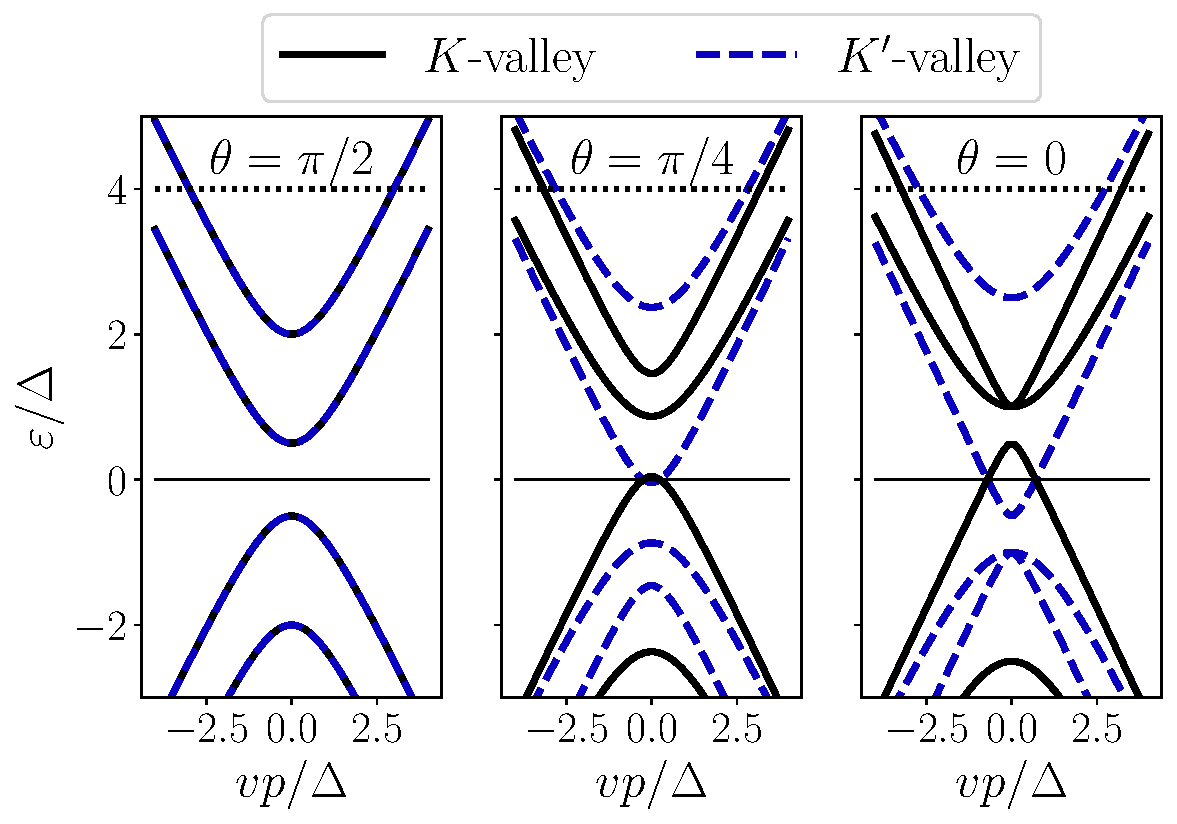
\includegraphics[width=\columnwidth]{{articles/misha_paper/fig2.pdf}}}
\caption{Electronic band structure of the honeycomb AFM model of Eq.~(\ref{chap03:eff}) for different orientations of the N\'eel vector ($n_z=\cos\theta$). Two-dimensional momenta $\bb{p}$ are measured with respect to the wave-vectors $\bm{K}$ and $\bm{K}^\prime$ that specify two nonequivalent valleys. Deviation of the N\'eel vector from the perpendicular-to-the plane configuration ($\theta=0$) lifts the valley degeneracy. We restrict our analysis to the metallic regime with Fermi energies corresponding to two Fermi surfaces per valley (an example is shown by a black dotted line). The energy scale $\Delta_{\text{sd}}$ characterizes the strength of $s$-$d$ exchange interaction.
}
\label{chap03:fig:spectrum}
\end{figure}
%%%%%%%%%

The nonequilibrium contributions $\delta\bb{s}^{\pm}$ originate from various forces applied to conduction electrons. One natural example is the electric field that not only induces an electric current in the sample but also contributes to $\delta\bb{s}^{\pm}$. The electric field can be further related to electric current by the resistivity tensor. The response of spin densities to electric current defines the so-called spin-orbit torques in Eqs.~(\ref{chap03:AFMEOM}) that we also compute.

Similarly, the response of $\delta\bb{s}^{\pm}$ to the time derivatives $\dot{\bb{n}}$ and $\dot{\bb{m}}$ describe various types of Gilbert damping induced by conduction electrons. Quite generally, such a response can be written in the form of a tensor
\be
\label{chap03:response}
\bpm 
\delta \bb{s}^{+}\\
\delta \bb{s}^{-}
\epm=
\bpm 
\hat{\alpha}_m & \hat{\alpha}_{mn}\\
\hat{\alpha}_{nm} & \hat{\alpha}_n
\epm
\bpm 
\dot{\bb{m}}\\
\dot{\bb{n}}
\epm,
\e
where all tensor components may themselves depend on the vectors $\bb{n}$ and $\bb{m}$. 

Gilbert dampings, in their original meaning, correspond to the contributions to $\delta\bb{s}^{\pm}$ that are symmetric under the time reversion. 
The terms that change sign should, more appropriately, be referred to as effective spin renormalizations. Both types of terms are, however, obtained from the microscopic analysis of the Gilbert damping tensors in Eq.~(\ref{chap03:response}) similarly to the case of ferromagnets \cite{ado_anisotropy_2019}.

Time reversion, mentioned above, applies exclusively to the Heisenberg model, while keeping the tight-binding model (a bath) non-reversed. In other words we do not reverse the electron scattering time $\tau$. Such a definition helps to identify the dissipative (even with respect to the time reversion) contributions to $\delta\bb{s}^{\pm}$ that describe Gilbert dampings. These contributions must, however, change sign under the transformation $\tau \to -\tau$, because spin densities $\bb{s}^\pm$ are always odd with respect to complete time reversion (the one which also includes that of the electron bath). We will see below, indeed, that all Gilbert dampings are proportional to the scattering time $\tau$ in the same way as the longitudinal conductivity does.  

Before we proceed with the microscopic analysis of $\delta\bb{s}^{\pm}$ for a particular model, it is instructive to draw some general consequences for Eqs.~(\ref{chap03:AFMEOM}) based on symmetry arguments in the case of collinear AFM with sublattice symmetry and spin-rotational invariance (i.\,e. for vanishing spin-orbit interaction).  

Assuming that deviations from the AFM ground state remain small we shall limit ourselves to the linear order in $\bb{m}$ in Eq.~(\ref{chap03:even}) and to the quadratic order in $\bb{m}$ in Eq.~(\ref{chap03:staggered}).  Thus, we shall retain terms up to linear order in $\bb{m}$ in the tensors $\hat{\alpha}_{m}$, $\hat{\alpha}_{nm}$, and $\hat{\alpha}_{mn}$ and terms up to quadratic order in $\bb{m}$ in $\hat{\alpha}_n$. 

Mixing tensors $\hat{\alpha}_{mn}$ and $\hat{\alpha}_{nm}$ must be odd in $\bb{m}$, which implies, for our precision, a linear in $\bb{m}$ approximation. As a result, the sublattice symmetry (the symmetry with respect to renaming $A$ and $B$) prescribes that the mixing tensors must also be linear in $\bb{n}$. In the absence of spin-orbit coupling we are also restricted by spin-rotation invariance that (together with the sublattice and time-reversion symmetries) dictates the following form of the Gilbert damping contributions to the non-equilibrium spin densities
\beml
\label{chap03:gen}
\begin{align}
\label{chap03:even}
\delta \bb{s}^{+} & = \alpha_m \dot{\bb{m}}  \!+\! \alpha'_m \bb{n}  \!\times\! (\bb{n} \!\times\! \dot{\bb{m}}) \!+\!\alpha_{mn}\bb{m}  \!\times\!  (\bb{n}  \!\times\!  \dot{\bb{n}}),\\
\delta \bb{s}^{-} &= \alpha_n \dot{\bb{n}} \!+\! \alpha'_n \bb{m}  \!\times\! (\bb{m} \!\times\! \dot{\bb{n}}) + \alpha_{nm} \bb{n}\!\times\!(\bb{m}\!\times\! \dot{\bb{m}}),
\label{chap03:staggered}
\end{align}
\eml
where all coefficients are assumed to be constants.  

It is easy to see that the vector forms $\bb{n}\times(\bb{m}\times\dot{\bb{n}})$ and $\bb{m}\times(\bb{n}\times \dot{\bb{m}})$, which could have respectively entered the spin densities $\delta\bb{s}^+$ and $\delta\bb{s}^-$, do not contribute to Eqs.~(\ref{chap03:AFMEOM}) in the precision explained above.  
Substitution of Eqs.~(\ref{chap03:gen}) into Eqs.~(\ref{chap03:AFMEOM}) gives 
\beml
\label{chap03:AFMEOM2}
\begin{align}
\label{chap03:ndot2}
&\dot{\bb{n}} = -\Omega\, \bb{n}\!\times\!\bb{m} +\bb{H}\!\times\!\bb{n}+\bar{\alpha}_m\,\bb{n}\!\times\!\dot{\bb{m}}+\alpha_n\,\bb{m}\!\times\! \dot{\bb{n}},\\
&\dot{\bb{m}} =\bb{H}\times\bb{m}+\alpha_n\,\bb{n} \times \dot{\bb{n}}+\bar{\alpha}_m \bb{m} \times \dot{\bb{m}} +\gamma (\bb{n}\times\bb{m})(\bb{n}\cdot\dot{\bb{m}}) - \alpha_n'm^2\bb{n}\times\dot{\bb{n}},
\label{chap03:mdot2}
\end{align}
\eml
where $\bar{\alpha}_m=\alpha_m\!-\!\alpha'_m$ and $\gamma=\alpha_{mn}\!+\!\alpha_{nm}\!+\!\alpha'_m\!-\!\alpha'_n$. Discarding the three last terms in Eq.~(\ref{chap03:mdot2}), which are all of the second order in $\bb{m}$, we indeed arrive at a set of Gilbert damping terms that is  widely used in the AFM literature \cite{Kamra2018,PhysRevMaterials.1.061401,Yuan_2019}. 

The symmetry consideration behind Eqs.~(\ref{chap03:AFMEOM2}) has essentially relied upon the spin-rotation invariance. This also implies $\alpha_n=0$ as has been pointed out in the introductory section. The coefficient $\alpha_m$ can, in turn, be finite and large, even in the absence of spin-orbit interaction. As we will show below, the presence of spin-orbit interaction does not only provide us with a finite $\alpha_n$ but also drastically change the symmetry structure of Eqs.~(\ref{chap03:AFMEOM2}). We will demonstrate that the onset of spin-orbit interaction strongly affects the coupling of the localized spin subsystem to the electron bath (described by the tight-binding model) resulting in a strong reduction in the ability of conduction electrons to flip spins in certain directions and, therefore, to impose a friction on magnetization dynamics. 

In the following, we turn to the microscopic analysis of the conductivity (Sec.~\ref{chap03:sec:cond}), spin-orbit torques (Sec.~\ref{chap03:sec:sot}) and Gilbert dampings (Sec.~\ref{chap03:sec:gd}) in a particular model of Rashba honeycomb AFM that has been put forward recently by some of the authors \cite{sumit2019}. Rashba spin-orbit interaction breaks spin-rotational invariance of the model by singling out the direction $\hat{\bb{z}}$ perpendicular to the 2D plane. We, therefore, investigate how such spin-rotation breaking manifests itself in the anisotropy of the abovementioned quantities.  

\section{Microscopic model}

For the sake of a microscopic analysis we adopt a sublattice symmetric $s$-$d$-like model of a 2D honeycomb antiferromagnet with Rashba spin-orbit coupling, that was used in the previous Chapter as well. The energy dispersion of this model is illustrated schematically in Fig.~\ref{chap03:fig:spectrum}.  
The low energy model for conduction electrons responsible for the dispersion in Fig.~\ref{chap03:fig:spectrum}, is described by an effective Hamiltonian (see Appendix ~\ref{chap03:sec:appa}) that in a valley-symmetric representation reads
\be
\label{chap03:eff}
H^\textrm{eff}= v\, \bb{p}\cdot\bb{\Sigma}+\tfrac{1}{2}\lambda\lt[\bb{\sigma}\times\bb{\Sigma}\rt]_{\hat{z}} - \Delta_{\text{sd}}\,\bb{n}\cdot\bb{\sigma}\,\Sigma_z\Lambda_z + V(\bb{r}).
\e
Here $\bb{\Sigma}$, $\bb{\Lambda}$, and $\bb{\sigma}$ are the vectors of Pauli matrices in sublattice, valley and spin space, respectively, $v$ is the characteristic Fermi velocity, while $\lambda$ and $\Delta_{\text{sd}}=JS$ are the energy scales characterizing the strength of Rashba spin-orbit coupling and $s$-$d$-like exchange energy, correspondingly. 

% The term $V(\bb{r})$ stands for a scalar Gaussian white-noise disorder potential, which is proportional to the unit matrix in sublattice, valley and spin space. The potential has a zero mean value $\la V(\bb{r}) \ra=0$ and is fully characterized by the pair correlator,
% \be
% \lt\la V(\bb{r}) V(\bb{r}') \rt\ra = 2\pi (\hslash v)^2 \alpha_\textrm{d}\;\delta(\bb{r}-\bb{r}'),
% \e
% where the angular brackets denote the averaging over disorder realizations. The dimensionless parameter $\alpha_\textrm{d}\ll 1$ quantifies the disorder strength. 

The disorder potential is responsible for a momentum relaxation of conduction electrons. Exchange interaction and spin-orbit scattering (or the scattering on a non-collinear configurations with $\bb{m}\neq 0$) enable coupling between localized angular momenta and kinetic momenta of electrons. Together these mechanisms form a channel to dissipate angular momentum of localized spins into the lattice. Thus, our model provides us with a microscopic framework to study dissipative quantities such as Gilbert dampings, anti-damping spin-orbit torques and conductivity that we compute below. We also note that the computation of spin-relaxation time can be directly related to our analysis of Gilbert damping \cite{manchon_spin_2017}. 

The spectrum of the model (\ref{chap03:eff}) with $V(\bb{r})=0$ consists of two electron and two hole branches for each of the valleys as illustrated in Fig.~\ref{chap03:fig:spectrum},
\beml
\label{chap03:spectrum}
\begin{align}
\label{chap03:spectrume}
\epsilon^e_{\pm,\varsigma}(p)&=\sqrt{v^2p^2+\Delta_{\text{sd}}^2\pm \varsigma\lambda\Delta_{\text{sd}} n_z+\lambda^2/4} \mp \lambda/2,\\
\epsilon^h_{\pm,\varsigma}(p)&=-\sqrt{v^2p^2+\Delta_{\text{sd}}^2\mp \varsigma\lambda\Delta_{\text{sd}} n_z+\lambda^2/4} \pm \lambda/2,
\end{align}
\eml
where $\varsigma=\pm$ is the valley index. All spectral branches are manifestly isotropic with respect to the direction of the electron momentum $\bb{p}$ irrespective of the N\'eel vector orientation (as far as $\bb{m}=0$). 

In order to limit the complexity of our microscopic analysis we restrict ourselves to the metallic regime that corresponds to the Fermi energy $\ep_F > \Delta_{\text{sd}}+\lambda$ above the minimum of the top electron branches, $\epsilon^e_{+,\varsigma}(p)$, as shown schematically in Fig.~\ref{chap03:fig:spectrum}. Note that the Fermi energy $\ep_F$ is counted in the model from the center of the AFM gap. 
We also focus on the limit of weak disorder $\ep_F \tau/\hslash\gg 1$ where $\tau = \hslash/(\pi\alpha_\textrm{d}\ep_F)$ stands for the electron scattering time. Also, in order to describe spin-orbit induced anisotropy we find it convenient to decompose the N\'eel vector (as well as the magnetization vector) to the in-plane and perpendicular-to-the-plane components as $\bb{n}= \bb{n}_\parallel+\bb{n}_\perp$, where $\bb{n}_\perp=n_z\hat{\bb{z}}$. 

\section{Conductivity}\label{chap03:sec:cond}
The electric conductivity in the metallic regime is dominated by electron diffusion. Despite the fact that the Fermi surface (line) is isotropic and does not depend on the direction of $\bb{n}_\parallel$, the conductivity appears to be weakly anisotropic with respect to in-plane rotations of the N\'eel vector due to the onset of spin-orbit interaction. 
In particular, for $n_z=0$ we find the diagonal conductivity components
\beml
\label{chap03:conductivity}
\begin{align}
\label{chap03:chap3:eq:long_cond}
&\sigma_{xx}= \frac{4e^2}{h}\,\frac{\ep_F \tau}{\hslash}\,\frac{\ep_F^2-\Delta_{\text{sd}}^2}{\ep_F^2+3\Delta_{\text{sd}}^2},\\
&\sigma_{yy}= \sigma_{xx}+\frac{4e^2}{h}\,\frac{\ep_F \tau}{\hslash}\, \frac{\ep_F^2}{\ep_F^2+\Delta_{\text{sd}}^2}
\frac{\lambda^2\Delta_{\text{sd}}^2}{\ep_F^4+\ep_F^2\Delta_{\text{sd}}^2+2\Delta_{\text{sd}}^4},
\end{align}
\eml
where the principal axes correspond to choosing $\hat{\bm{x}}$ direction along $\bb{n}_\parallel$ (see Fig.~\ref{chap03:fig:lattice}). In the deep metal regime, and for a general direction of $\bb{n}$, this anisotropy is evidently small
\be
\label{chap03:ani}
\frac{\rho_{xx}-\rho_{yy}}{\rho_{xx}+\rho_{yy}}=\frac{\lambda^2\Delta_{\text{sd}}^2}{\ep_F^4}(1-n_z^2), \quad \ep_F\gg \lambda+\Delta_{\text{sd}},
\e
where $\rho_{aa}=1/\sigma_{aa}$ is the corresponding resistivity tensor component. We note that the anomalous Hall conductivity is identically vanishing in the model of Eq.~(\ref{chap03:eff}). 

The results of Eq.~(\ref{chap03:conductivity}) and all subsequent results of our Chapter are technically obtained from linear response Kubo formulas evaluated in the diffusive approximation (ladder diagram summation). The details of these calculations can be found in Appendixes~\ref{chap03:sec:appb}, \ref{chap03:sec:appc}, and \ref{chap03:sec:appd}. 

\section{Spin-orbit torque}\label{chap03:sec:sot}

Before proceeding with the microscopic analysis of Gilbert damping we shall discuss the effects of spin-orbit induced anisotropy for spin-orbit torques in the model of Eq.~(\ref{chap03:eff}). Since this anisotropy appears to be weak in the metal regime, we shall touch on it only briefly. 

As was already mentioned, the spin-orbit torques originate in the response of nonequilibrium spin polarizations $\delta\bb{s}^\pm$ to electric current. Technically, we compute first the response of $\delta\bb{s}^\pm$ to electric field and, then, express the electric field in terms of 2D electric current density $\bb{j}$ using the conductivity tensor of Eq.~(\ref{chap03:conductivity}).

A straightforward computation of such a response gives $\delta\bb{s}^-=0$ (see Appendixes~\ref{chap03:sec:appb} and \ref{chap03:sec:appc} for more detail) and 
\begin{multline}
\label{chap03:sp}
\delta\bb{s}^+= a(n_z^2)\;\hat{\bb{z}}\times \bb{j} + b(n_z^2)\, \bb{n}_\parallel\times(\bb{n}_\parallel\times \lt(\hat{\bb{z}}\times \bb{j}\rt))\\
+ c(n_z^2)\, \bb{n}_\parallel \times(\bb{n}_\perp\times \lt(\hat{\bb{z}}\times \bb{j}\rt)),
\end{multline}
where the coefficients $a$, $b$ and $c$ do generally depend on $n_z^2=1-n_x^2-n_y^2$ and are shown in Fig.~\ref{chap03:fig:abc}. 
It is appropriate to recall here that the computation of the responses from the model of Eq.~(\ref{chap03:eff}) refers to the case when $\bb{m}=0$. The symmetry form of Eq.~(\ref{chap03:sp}) in this case has been also established recently from numerical simulations \cite{sumit2019}.

Importantly, the first term in the right-hand side of Eq.~(\ref{chap03:sp}) represents the well-known Rashba-Edelstein effect \cite{edelstein_spin_1990}, while the other two terms represent higher harmonics of the same field-like effect that arise due to spin-rotation symmetry breaking. Anti-damping like torques (that are even under time-reversal) are vanishing in the model due to the valley symmetry constraint. This symmetry reads $\Lambda_x H[\bb{n}] \Lambda_x = H[-\bb{n}]$, from which it follows that the response of $\delta\bb{s}^+$ to charge current must be an even function of $\bb{n}$. 

The behavior of the coefficients $a$, $b$ and $c$ as a function of $n_z$ is illustrated in Fig.~\ref{chap03:fig:abc} for two different choices of the Fermi energy. For in-plane N\'eel vector orientations ($n_z=0$) we find 
\beml
\label{chap03:SOT}
\begin{align}
&a=a_0 \frac{1+3\delta^2}{1+2\bar{\lambda}^2\delta^2+\delta^4-2\delta^6},\\
&b=2\, a\,\delta^2\,\frac{1-2\bar{\lambda}^2-4\delta^2+\delta^4}{1+2\delta^2-3\delta^4},\\
&c=-2\, a\,\delta^2\,\frac{1+2\bar{\lambda}^2\delta^2-2\delta^2-3\delta^4-4\delta^6}{1+4\delta^2+5\delta^4+6\delta^6},
\end{align}
\eml
where
\be
a_0=\frac{\mathcal{A}J}{e\hslash v}\,\frac{\lambda}{\ep_F}, \qquad \bar{\lambda}=\frac{\lambda}{\ep_F},\qquad\delta=\frac{\Delta_{\text{sd}}}{\ep_F}.
\e
In the metal regime, $\ep_F\gg \lambda+\Delta_{\text{sd}}$, the results of Eqs.~(\ref{chap03:SOT}) are reduced to 
\be
\label{chap03:SOTlargeE}
a=\frac{\mathcal{A}J}{e\hslash v}\,\frac{\lambda}{\ep_F}, \qquad b=-c=2\,\frac{\mathcal{A}J}{e\hslash v}\,\frac{\lambda}{\ep_F}
\lt(\frac{\Delta_{\text{sd}}}{\ep_F}\rt)^2.
\e
One can, therefore, see that the high harmonics terms (proportional to $b$ and $c$) become irrelevant in the metal regime.  

Vanishing response of the staggered polarization, $\delta\bb{s}^-=0$, for the model of Eq.~(\ref{chap03:eff}) is a simple consequence of the sublattice symmetry. As shown below the presence of a finite, though small, $\bb{m}$ breaks such a symmetry and leads to a finite $\delta\bb{s}^-$. Taking into account a linear in $\bb{m}$ term in the Hamiltonian is also necessary to obtain finite mixed Gilbert damping tensors $\hat{\alpha}_{nm}$ and $\hat{\alpha}_{mn}$ in Eq.~(\ref{chap03:response}).   

%%%%%%%%%%%%
%%% figure 3: 
%%%%%%%%%%%%
\begin{figure}
\centering
\centerline{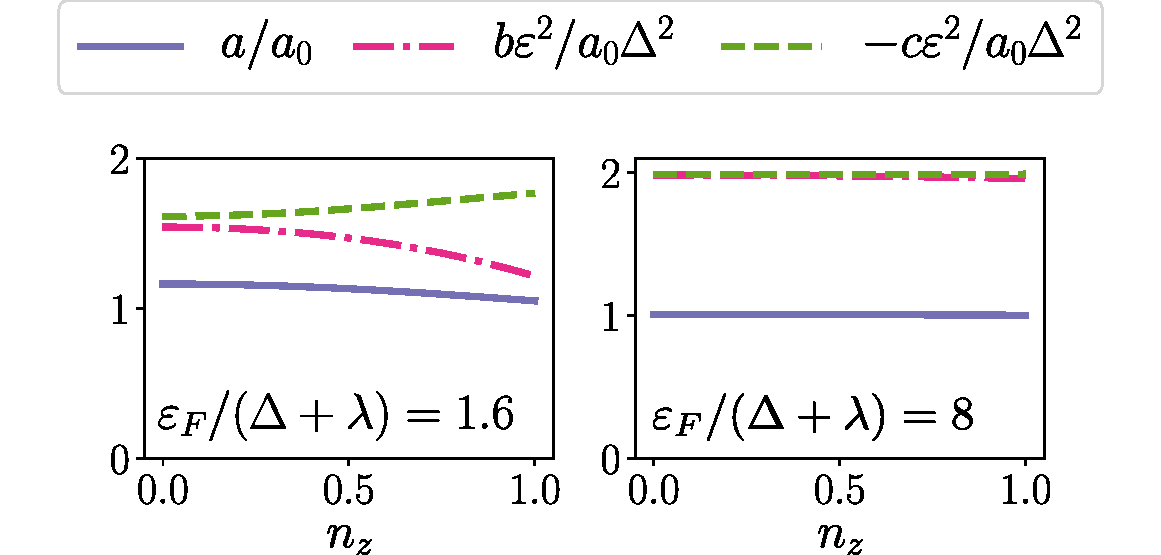
\includegraphics[width=\columnwidth]{{articles/misha_paper/fig3.pdf}}}
\caption{The coefficients $a$, $b$, and $c$ in Eq.~(\ref{chap03:sp}) as a function of the direction of the N\'eel vector, $n_z=\cos\theta$, for two different Fermi energies: $\ep_F=4\Delta_{\text{sd}}$ (left panel) and  $\ep_F=16\Delta_{\text{sd}}$ (right panel). We use $\lambda=1.5\Delta_{\text{sd}}$.  For $n_z=0$ the results correspond to Eqs.~(\ref{chap03:SOT}). 
}
\label{chap03:fig:abc}
\end{figure}
%%%%%%%%%

A low-energy model that takes into account finite magnetization vector reads (see also Appendix~\ref{chap03:sec:appd})
\be
\label{chap03:full}
H=H^\textrm{eff}-\Delta_{\text{sd}}\,\bb{m}\cdot\bb{\sigma},
\e
where $H^\textrm{eff}$ is given by Eq.~(\ref{chap03:eff}). The conductivity tensor does not acquire a linear in $\bb{m}$ terms in the leading order with respect to the large metal parameter $\ep_F\tau/\hslash$, because the anomalous Hall effect remains subleading with respet to the metal parameter. Similarly, the result of Eq.~(\ref{chap03:sp}) is not affected by the linear in $\bb{m}$ corrections. 

However, the direct computation of the staggered polarization response (in the linear order with respect to $\bb{m}$) gives rise to a finite result. In the limit of large Fermi energy $\ep_F\gg \lambda+\Delta_{\text{sd}}$, we find 
\begin{multline}
\delta\bb{s}^-= \frac{\mathcal{A}J}{e\hslash v}\,\frac{\lambda}{\ep_F}
\lt(\frac{\Delta_{\text{sd}}}{\ep_F}\rt)^2\,
\Big[2\,\bb{n}_{\perp} \!\times\!(\bb{m}_{\perp} \!\times\! (\hat{\bb{z}}\!\times\!\bb{j}))
\\
+2\,\bb{m}_{\parallel} \!\times\!(\bb{n}_{\perp} \!\times\! (\hat{\bb{z}}\!\times\!\bb{j})) -3\,\bb{n}_{\parallel}\!\times\! (\bb{m}_{\perp}\! \times\! (\hat{\bb{z}}\!\times\!\bb{j}))\n \Big],
\label{chap03:stagg}
\end{multline}
where the overall strength of the effect is again of the order of the coefficients $b$ and $c$. This makes the effects of nonequilibrium staggered polarization (including the celebrated N\'eel spin-orbit torque) irrelevant in the metal regime. Indeed, staggered polarization can hardly be induced by electrons with wavelengths that strongly exceed the distance between $A$ and $B$ sublattices.  

The results of Eqs.~(\ref{chap03:sp}), (\ref{chap03:SOT}) clearly suggest that the only torques surviving in the large energy limit are those related to non-equilibrium polarization $\delta\bb{s}_+=a_0 \,\hat{\bb{z}}\times\bb{j}$, which is nothing but the standard Rashba-Edelstein effect \cite{edelstein_spin_1990}. These torques have a form $\bb{T}_n= a_0 \,\bb{n}\times(\hat{\bb{z}}\times\bb{j})$ in the right-hand side of Eq.~(\ref{chap03:ndot}) and $\bb{T}_m= a_0 \,\bb{m}\times(\hat{\bb{z}}\times\bb{j})$ in the right-hand side of Eq.~(\ref{chap03:mdot}). The anisotropy of torques is, however, irrelevant in this limit.  

\section{Gilbert damping}\label{chap03:sec:gd}

Surprisingly, the situation is different when we consider Gilbert damping terms. In this case we find that the giant anisotropy of Gilbert damping persists to arbitrarily large Fermi energy as soon as spin orbit energy $\lambda$ exceeds $\hslash/\tau$. The latter condition ensures that the scattering between spin-split subbands is suppressed. 

The direct computation of the Gilbert damping tensors for $\lambda\gg \hslash/\tau$ gives
\beml
\label{chap03:gilbert}
\begin{align}
&\delta\bb{s}^+= \alpha_m^\parallel\,\dot{\bb{m}}_\parallel + \gamma \bb{\Gamma}_{mm}+ \gamma\bb{\Gamma}_{mn},\\
&\delta\bb{s}^-= \alpha_n^\perp\,\dot{\bb{n}}_\perp +\gamma \bb{\Gamma}_{nm}+\gamma \bb{\Gamma}_{nn},
\end{align}
\eml
where the terms $\Gamma_{ab}$ contain various vector forms. 

Far in the metal regime, $\ep_F\gg \lambda+\Delta_{\text{sd}}$, we find
\beml
\label{chap03:coeffGD}
\begin{align}
&\alpha_m^\parallel= 2\,\frac{\ep_F\tau}{\hslash}\;\frac{\mathcal{A} J^2 S}{\pi\hslash^2v^2}\; \lt[1-\frac{\Delta_{\text{sd}}^2}{\ep_F^2}(2+n^2_z) + \dots\rt],\\
&\alpha_n^\perp = \frac{\ep_F\tau}{\hslash}\;\frac{\mathcal{A} J^2 S}{\pi\hslash^2v^2} \,\lt[\lt(\frac{\lambda}{\ep_F}\rt)^2+\dots\rt],\\
&\gamma= 2\,\frac{\ep_F\tau}{\hslash}\;\frac{\mathcal{A} J^2 S}{\pi\hslash^2v^2}\,\lt[\lt(\frac{\Delta_{\text{sd}}}{\ep_\textrm{F}}\rt)^2+\dots\rt],
\end{align}
\eml
while the vectors forms $\Gamma_{ab}$ can be written as
\beml
\begin{align}
\bb{\Gamma}_{mm}=&\,
\bb{n}\!\times\!(\bb{n}\!\times\!\dot{\bb{m}}) + \bb{n}_\parallel\!\times\!(\bb{n}_\parallel\!\times\!\dot{\bb{m}}_\parallel)  
- 2 \bb{n}_\parallel\!\times\!(\bb{n}_\parallel\!\times\!\dot{\bb{m}}_\perp),\\
\bb{\Gamma}_{mn}=&\,
\bb{n}\!\times\!(\bb{m}_\parallel\!\times\!\dot{\bb{n}}_\perp) 
- \bb{m}_\perp\!\times\!(\bb{n}_\parallel\!\times\!\dot{\bb{n}}_\perp)
+\bb{n}_\perp\!\times\!(\bb{m}_\perp\!\times\!\dot{\bb{n}}_\parallel) \n\\
&- \bb{n}_\parallel\!\times\!(\bb{m}_\parallel\!\times\!\dot{\bb{n}}_\parallel)
- 3\bb{m}_\perp\!\times\!(\bb{n}_\perp\!\times\!\dot{\bb{n}}_\parallel),\\
\bb{\Gamma}_{nm}=&\,2\bb{n}_\parallel\!\times\!(\bb{m}_\parallel\!\times\!\dot{\bb{m}}_\perp)+ 
2\bb{m}_\parallel\!\times\!(\bb{n}_\perp\!\times\!\dot{\bb{m}}_\parallel)
-\bb{n}_\perp\!\times\!(\bb{m}_\perp\!\times\!\dot{\bb{m}})\n\\
&+2 \bb{m}_\perp\!\times\!(\bb{n}\!\times\!\dot{\bb{m}})
+ \bb{m}_\parallel\!\times\!(\bb{n}\!\times\!\dot{\bb{m}}_\perp) 
- \bb{m}_\perp\!\times\!(\bb{n}_\perp\!\times\!\dot{\bb{m}}_\parallel),\\
\bb{\Gamma}_{nn}=&\,-\bb{m}\times(\bb{n}\times\dot{\bb{n}}_\parallel).
\end{align}
\eml
Thus, we see from Eqs.~(\ref{chap03:coeffGD}) that the coefficients $\alpha_n^{\perp}$ and $\gamma$ are vanishingly small in the metal regime. Moreover, in the limit $\ep_F\gg \Delta_{\text{sd}}$ the only non-vanishing contributions to Gilbert dampings are given by the first terms on the right-hand sides of Eqs.~(\ref{chap03:gilbert}) that are manifestly anisotropic.

%The forms entering $\bb{\Gamma}_{mm}$, $\bb{\Gamma}_{mn}$, $\bb{\Gamma}_{nm}$, and $\bb{\Gamma}_{nn}$ are obtained, respectively, from the analysis of the tensors $\hat{\alpha}_m$, $\hat{\alpha}_{nm}$, $\hat{\alpha}_{mn}$, and $\hat{\alpha}_n$ with the help of the first order perturbation theory in $\bb{m}$.

The onset of spin-orbit interactions therefore makes Gilbert dampings ultimately anisotropic, also in the deep metal regime. This is in contrast to conductivity and spin-orbit torques that are quickly becoming isotropic in the metal limit. 
For $\ep_F\gg \lambda+\Delta_{\text{sd}}$, we find the well known Landau-Lifshitz-Gilbert equations
\begin{align}
&\dot{\bb{n}} = -\Omega\, \bb{n}\!\times\!\bb{m} +\bb{H}\!\times\!\bb{n}+\bar{\alpha}^\parallel_m\,\bb{n}\!\times\!\dot{\bb{m}}_\parallel+\alpha_n^\perp\,\bb{m}\!\times\! \dot{\bb{n}}_\perp,\n\\
&\dot{\bb{m}} =\bb{H}\times\bb{m}+\alpha_n^\perp\,\bb{n} \times \dot{\bb{n}}_\perp
+\bar{\alpha}_m^\parallel \bb{m} \times \dot{\bb{m}}_\parallel,
\label{chap03:AFMEOM3}
\end{align}
where we again omit terms that originate e.\,g. from magnetic anisotropy of the AFM. 
Eqs. (\ref{chap03:AFMEOM3}) are clearly different from Eqs.~(\ref{chap03:AFMEOM2}) derived on the basis of symmetry analysis in the absence of spin-orbit interaction. 

The very pronounced, highly anisotropic Gilbert damping terms in the Landau-Lifshitz-Gilbert equations of Eqs.~(\ref{chap03:AFMEOM3}) represent the main result of our Chapter. The phenomenon of the giant Gilbert damping anisotropy in the 2D AFM clearly calls for a qualitative understanding that we provide in Sec.~\ref{chap03:sec:qual}.

\section{Qualitative consideration}\label{chap03:sec:qual}

The results of Eqs.~(\ref{chap03:gilbert}), (\ref{chap03:coeffGD}) suggest that the anisotropy of Gilbert damping is most pronounced in the metal limit, $\ep_F\gg \Delta_{\text{sd}}+\lambda$ as far as $\lambda \tau/\hslash \gg 1$. In particular, certain spin density responses are vanishing in this limit. One of them is the response of the average spin density $\delta s_z^+$ to $\dot{m}_z$ that is defined by the tensor component $\alpha^{zz}_m$ in Eq.~(\ref{chap03:response}). The other four vanishing tensor components $\alpha^{xx}_n$, $\alpha^{xy}_n$, $\alpha^{yx}_n$ and $\alpha^{yy}_n$ correspond to the responses of the in-plane staggered spin densities $\delta s_{x}^-$ and $\delta s_{y}^-$ to $\dot{n}_x$ and $\dot{n}_y$.  

It is important to stress that the component $\alpha^{zz}_m$ is not only finite but also quite large in the absence of spin-orbit interaction, i.\,e. for $\lambda=0$. It is, therefore, instructive to understand how the onset of spin-orbit interaction may cancel $\alpha^{zz}_m$ response and lead to the conservation of $z$ projection of magnetization vector.  

Such a qualitative understanding can be achieved by considering the Kubo-Greenwood formula for $\alpha^{zz}_m$ for the model 
of Eq.~(\ref{chap03:full}) in the limit $\Delta_{\text{sd}}\to 0$ and $\tau\to \infty$, 
\be
\label{chap03:Kubo}
\alpha^{zz}_m \propto \s_{\bb{p}}\!\!\s_{s,s'=\pm} \!|\la \Psi_{\bb{p},s}| \sigma_z |\Psi_{\bb{p},s'}\ra |^2
\delta(\ep_\textrm{F}-\epsilon^{e}_{p,s})\delta(\ep_\textrm{F}-\epsilon^{e}_{p,s'}),
\e
where $\epsilon^e_{p,\pm}=\sqrt{v^2p^2+\lambda^2/4}\mp\lambda/2$ correspond to the two electronic branches of Eq.~(\ref{chap03:spectrume}) that are evidently valley degenerate in the limit $\Delta_{\text{sd}}\to 0$. 

The states $\Psi_{\bb{p},s}$ are simply the eigenstates of the Hamiltonian $H_0 = v\bb{p}\cdot\bb{\Sigma}+(\lambda/2) \lt[\bb{\sigma}\times\bb{\Sigma}\rt]_z$,
\be
H_0 =
\bpm
0 & 0 & v(p_x \!-\!i p_y) & 0\\
0 & 0 & -i \lambda & v(p_x\!-\!i p_y) \\
v(p_x\!+\!i p_y) & i\lambda & 0 & 0\\
0 & v(p_x\!+\!i p_y) & 0 & 0
\epm,
\e
that can be explicitly written as
\be
\Psi_{\bb{p},\pm}=
\frac{1}{2\sqrt{v^2p^2\mp\lambda \epsilon^e_\pm/2}} \bpm vp\, e^{-i \phi}\\ \pm i \epsilon^e_\pm\\ \epsilon^e_\pm\\ \pm i v p\, e^{i \phi}\epm,
\e
where we have used $p_x=p\cos\phi$, $p_y=p\sin\phi$. 

One may notice that $\la \Psi_{\bb{p},s}| \sigma_z |\Psi_{\bb{p},s}\ra =0$ for any value of $\lambda$ suggesting that the response function $\alpha^{zz}_m$ in Eq.~(\ref{chap03:Kubo}) is vanishing. This is, however, not the case for $\lambda=0$. Indeed, in the absence of spin-orbit interaction the electron branches become degenerate $\epsilon^e_{p,\pm}=v p$ such that the in-plane spin-flip processes contribute to the Kubo formula,
\be
\lt.\la \Psi_{\bb{p},+}| \sigma_z |\Psi_{\bb{p},-}\ra\rt|_{\lambda=0}=\lt.\la \Psi_{\bb{p},-}| \sigma_z |\Psi_{\bb{p},+}\ra\rt|_{\lambda=0}=1.
\e
These processes are exactly the ones responsible for a finite Gilbert damping component $\alpha^{zz}_m$ in the absence of spin-orbit interaction. The spin-orbit induced splitting of the subbands  forbids these spin-flip processes as soon as $\lambda\tau/\hslash \gg 1$  and leads to a giant anisotropy of Gilbert damping in the metal limit. Indeed, the other elements of the Gilbert damping tensor $\alpha^{xx}_m$ and  $\alpha^{yy}_m$ remain finite irrespective of the subband splitting,
\be
\la \Psi_{\bb{p},\pm}| (\sigma_x+i\sigma_y) |\Psi_{\bb{p},\pm}\ra=\frac{\pm i v\,p\,e^{i\phi}}{\sqrt{v^2p^2+\lambda^2/4}}.
\e
One can further show that for $\lambda=0$ the entire Gilbert damping tensor $\hat{\alpha}_m$ becomes isotropic $\hat{\alpha}^{xx}_m=\hat{\alpha}^{yy}_m=\hat{\alpha}^{zz}_m$ as it have been expected on the basis of the symmetry analysis. 

Very similar physics is also responsible for the anisotropy of the tensor $\hat{\alpha}_n$. It is worth noting that the same type of anisotropy is known to take place in the limit of large spin-orbit interaction in 2D Rashba ferromagnets \cite{ado_anisotropy_2019}. Spin-orbit induced anisotropy of Gilbert damping plays, however, a lesser role in 2D ferromagnets due to the much stricter constraint on the single magnetization vector.  A less restricted dynamics of $\bb{m}$ and $\bb{n}$ vectors make the Gilbert damping anisotropy play a bigger role in 2D AFMs. 

Indeed, it can be directly seen from Eqs.~(\ref{chap03:AFMEOM3}) that a nonequilibrium state with  $\bb{m}=m \hat{\bb{z}}$ and $\bb{n}=\bb{n}_\parallel$ becomes undamped in the absence of external field $\bb{H}=0$. Such a state corresponds to the undamped N\'eel vector precession around $\hat{\bb{z}}$ axis with a frequency given by $J_\textrm{ex} m$. The state clearly survives in the presence of easy plane magnetic anisotropy in the AFM. We believe that such a phenomenon remains to be rather generic for a variety of 2D or layered AFM systems with strong spin-orbit coupling of Rashba type. 

\section{Conclusions}

In this Chapter, we demonstrate that the presence of sufficiently strong spin-orbit coupling $\lambda\tau/\hslash \gg 1$ results in the ultimate anisotropy of the Gilbert damping tensor in the metal regime, $\ep_F\gg\Delta_{\text{sd}}+\lambda$.  One can trace the phenomenon to the spin-orbit induced splitting of Fermi surfaces that forbids scattering processes that are responsible for the relaxation of certain magnetization and N\'eel vector components. 

We also demonstrate that a finite in-plane projection $\bb{n}_\parallel$ of the N\'eel vector is responsible for a weak anisotropy of conductivity and spin-orbit torques for Fermi energies approaching the band edge, $\ep_F \sim \Delta_{\text{sd}}+\lambda$. This anisotropy is, however, absent in the metallic regime. 

Gilbert damping is, however, isotropic in the absence of spin-orbit interaction as it is required by symmetry considerations. Thus, we demonstrate that the onset of Rashba spin-orbit interaction in 2D or layered AFM systems leads to a giant anisotropy of Gilbert damping in the metallic regime. The physics of this phenomenon originates in spin-orbit induced splitting of the electron subbands that destroys a particular decay channel for magnetization and leads to undamped precession of the N\'eel vector. The phenomenon is based on the assumption that other Gilbert damping channels  (e.\,g. due to phonons) remain suppressed in the long magnon wavelength limit that we consider. The predicted giant Gilbert damping anisotropy may have a profound impact on the N\'eel vector dynamics in a variety of 2D and layered AFM materials. 

% % \begin{acknowledgments}
% % We are thankful to I.\,Ado, H.\,Gomonay and J.\,Sinova for fruitful discussions. This research was supported by the JTC-FLAGERA Project GRANSPORT.  D.Y. and M.T. acknowledge the support from the Russian Science Foundation Project No. 17-12-01359. A.P. acknowledges support from the Russian Science Foundation Project 18-72-00058. The work of D.Y. was also supported by the Swedish Research Council (Vetenskapsr{\aa}det, 2018-04383). M.T. is especially thankful to the KITP visitor program ``Spintronics Meets Topology in Quantum Materials''. O.E. acknowledges support from the Swedish Research Council (Vetenskapsr{\aa}det) and the Knut and Alice Wallenberg foundation.
% % \end{acknowledgments}

% % \appendix


